\documentclass[anonymous]{iopjournal}

% Packages
\usepackage[T1]{fontenc}
\usepackage[utf8]{inputenc}
\usepackage{amsmath,amssymb}
\usepackage{graphicx}
\usepackage{booktabs}
\usepackage{array}
\usepackage{tabularx}
\usepackage{threeparttable}
\usepackage{enumitem}
\usepackage{microtype}
\usepackage[section]{placeins}
\usepackage{float}
\usepackage{needspace}
\usepackage{siunitx}
\usepackage{url}

% Formatting controls
\graphicspath{{figures/}}

\setlength{\parindent}{1.5em}
\setlength{\parskip}{0pt}
\raggedbottom

% Float placement tuned to keep figures/tables near their discussion while
% using page space efficiently.
\setcounter{topnumber}{4}
\setcounter{bottomnumber}{3}
\setcounter{totalnumber}{7}
\renewcommand{\topfraction}{0.95}
\renewcommand{\bottomfraction}{0.90}
\renewcommand{\textfraction}{0.05}
\renewcommand{\floatpagefraction}{0.80}
\setlength{\textfloatsep}{10pt plus 2pt minus 3pt}
\setlength{\floatsep}{8pt plus 2pt minus 2pt}
\setlength{\intextsep}{8pt plus 2pt minus 2pt}
\setlength{\abovecaptionskip}{5pt}
\setlength{\belowcaptionskip}{0pt}

\setlist[itemize]{topsep=2pt,itemsep=1pt,parsep=0pt,leftmargin=*}
\setlist[enumerate]{topsep=2pt,itemsep=1pt,parsep=0pt,leftmargin=*}

\sisetup{
  detect-all,
  per-mode=symbol,
  range-phrase=--,
  range-units=single
}

% Placeholder-safe figure command.
% This prevents the document from failing if a figure is missing.
\newcommand{\safeinclude}[2][]{%
  \IfFileExists{figures/#2}{%
    \includegraphics[#1]{figures/#2}%
  }{%
    \fbox{%
      \begin{minipage}[c][0.18\textheight][c]{0.88\linewidth}
      \centering
      \vspace{0.5em}
      \textbf{Figure file missing}\\[0.3em]
      Upload \texttt{\detokenize{figures/#2}}
      \vspace{0.5em}
      \end{minipage}
    }%
  }%
}

% Compact table column types.
\newcolumntype{Y}{>{\raggedright\arraybackslash}X}
\newcolumntype{L}[1]{>{\raggedright\arraybackslash}p{#1}}

% Manuscript metadata
\begin{document}

\articletype{Paper}

\title{A Computational Image-to-Mesh Pipeline for Cardiac Vascular Segmentation and Bioprinting-Oriented STL Generation from CT Angiography}

\author{[Author information removed for double-anonymous review]}

\affil{[Affiliation information removed for double-anonymous review]}

\begin{abstract}
Vascularization is a central challenge in engineering thick tissues because of the lack of reliable perfusion networks. Patient-specific vascular geometries from medical imaging may support bioprinting applications, but converting clinical scans into printable three-dimensional models requires multiple processing steps such as segmentation, mesh generation, repair, and quality control. We present an image-to-mesh pipeline that converts contrast-enhanced cardiac computed tomography (CT) angiography into vascular models relevant to future biofabrication workflows. The pipeline consists of (Phase A) a MONAI/PyTorch-based coronary vessel segmentation model and (Phase B) a post-processing stage that converts segmentations into stereolithography (STL) meshes. Phase A uses a three-dimensional Attention U-Net trained on the public ImageCAS dataset with a predefined 700/50/250 train/validation/test split. Preprocessing standardized image orientation, voxel spacing, intensity values, and training patches. The model was evaluated on the 250-case held-out test set, achieving a mean Dice@0.5 of 0.7878 (95\% CI 0.7820-0.7935; median 0.7934), a centreline Dice (clDice) score of 0.8695, and valid predictions for all test cases. The clDice advantage over Dice and HD95 was confirmed by a paired case-level bootstrap ($\Delta|\rho| = 0.118$, 95\% CI 0.054-0.183). Phase B generated repaired STL meshes that met the combined watertight and zero-detected-non-manifold-edge criterion in 91.2\% of cases. Topology-aware segmentation accuracy was more strongly associated with reduced mesh fragmentation than voxel-overlap accuracy, with clDice showing a stronger correlation with connected-component count ($\rho=-0.49$) than Dice ($\rho=-0.37$). The pipeline provides a reproducible route from coronary CTA to spatially faithful vascular STLs with quantified geometric quality control, and defines the specific fabrication-readiness gaps that physical printing must close.

\end{abstract}

\vspace{0.8em}
\keywords{3D bioprinting, vascularization, cardiac computed tomography angiography, coronary artery segmentation, 3D U-Net, Attention U-Net, MONAI, PyTorch, STL generation, mesh processing, biofabrication, patient-specific modeling}
\date{}

% =========================================================
\section{Introduction}
% =========================================================

Vascularization is a major issue in tissue engineering and biofabrication. Thick tissues need connected perfusable networks for oxygen delivery, nutrient transport, and waste removal. Without those networks, constructs cannot transport oxygen and nutrients and lose viability \cite{murphy2014,lovett2009,rouwkema2016,oconnor2022}. Cardiovascular disease remains the leading global cause of mortality \cite{who,tsao2023}, and engineered cardiac tissues are a long-term motivation for vascularized biofabrication. In cardiac tissue engineering, this challenge is especially important because cardiac tissues require precise structural organization and sustained perfusion \cite{murphy2020,noor2019,wu2023}.

Recent advances in extrusion-based bioprinting and freeform reversible embedding of suspended hydrogels (FRESH) have largely expanded the capabilities of soft, perfusable geometries that can be fabricated \cite{kolesky2014,ozbolat2016,hinton2015}. However, converting patient imaging data into fabrication-oriented anatomical models remains challenging. Clinical CTA contains spatial information that may be useful for patient-specific vascular templates, but preparing those data for fabrication typically requires multiple separate steps: image preprocessing, segmentation, manual correction, mesh extraction, smoothing, repair, quality control, and export.

Most medical image segmentation studies evaluate models primarily through voxelwise overlap metrics. For biofabrication, that is not sufficient. A vessel mask with a desired Dice score may still be unsuitable for real-world outputs if it contains discontinuous branches, non-manifold surfaces, geometric misalignment, or wall features that are too thin for stable bioprinting. As a result, segmentation performance and bioprinting-readiness are considered to be related but separate objectives.

This study presents a computational pipeline that addresses that gap. The goal is not only to segment coronary vascular anatomy from cardiac CTA, but also to convert segmentation outputs into geometrically consistent STL models for later fabrication-oriented review. First, the pipeline organizes a CTA-to-mesh workflow into reproducible Phase A and Phase B stages. Second, it connects conventional volumetric segmentation with mesh-generation and quality-control outputs. Third, it defines a computational scope in which vascular models are evaluated for geometric and mesh-based fabrication readiness rather than physical printing, perfusion, or biological function. By pairing full-cohort segmentation evaluation (including the topology-aware clDice) with cohort-level computational mesh-quality and fabrication-readiness checks, and by measuring the per-case association between the two, the study addresses image-derived vascular modeling as a coupled segmentation-to-geometry problem rather than a segmentation-only task. The analysis shows that centerline-aware segmentation accuracy predicts mesh connectivity more strongly than voxel overlap does.

% =========================================================
\section{Background and Related Work}
% =========================================================

Biofabrication has increasingly focused on vascularized constructs because perfusion is fundamental to the viability of larger engineered tissues \cite{groll2016,lovett2009,rouwkema2016,oconnor2022}, with applications in cardiac, musculoskeletal, and other regenerative contexts \cite{yang2023}. Patient-specific cardiac bioprinting studies have shown the promise of anatomically tailored tissues and perfusable patches, but maintaining vascular hierarchies remains difficult \cite{noor2019,wu2023,alonzo2019}. Extrusion-based printing is mostly robust and versatile, whereas FRESH and related embedded approaches improve handling of soft, freeform geometries \cite{ozbolat2016,hinton2015}.

On the imaging side, deep learning has become a major framework for biomedical segmentation. U-Net established the encoder-decoder design that has become standard in medical image analysis, and 3D U-Net extended that structure to volumetric data \cite{ronneberger2015,cicek2016}. Attention-gated variants improve localization of relevant structures in complex images \cite{oktay2018}. Frameworks such as nnU-Net and MONAI have further advanced reproducible development of volumetric pipelines \cite{isensee2021,cardoso2022}.

For coronary CTA specifically, public datasets have historically been limited, which has made comparisons across studies difficult. ImageCAS helps address that problem by providing a large-scale public benchmark for coronary artery segmentation \cite{zeng2023}. More recent work on ImageCAS has reported coronary segmentation performance using Dice, sensitivity, precision, and HD95, demonstrating the value of reporting multiple complementary metrics rather than Dice alone \cite{huang2025}. Nevertheless, even accurate CTA segmentation is not necessarily equivalent to fabrication readiness. Once a segmentation is produced, volumetric masks still require mesh extraction, geometric validation, smoothing, repair, and topology-aware quality checks before they can be considered as accurate fabrication geometry \cite{lorensen1987,lewiner2003,taubin1995}.

The gap addressed here therefore lies at the interface between medical image analysis and biofabrication. Prior work has advanced segmentation, bioprinting, or mesh processing in isolation. Fewer studies explicitly connect patient-specific CTA segmentation to print-oriented vascular model generation within a single workflow.

% =========================================================
\section{Methods}
% =========================================================

\subsection{Pipeline overview}

The proposed workflow converts cardiac CTA into bioprinting-oriented three-dimensional geometry through two connected phases: (i) automated coronary vascular segmentation and (ii) print-aware postprocessing and STL generation. An overview is shown in Figure~\ref{fig:pipeline}. The first stage takes preprocessed CTA volumes and produces voxelwise vascular predictions. The second stage validates image geometry, standardizes masks or probability maps, reconstructs a surface mesh, improves mesh quality, exports STL models, and generates quality-control outputs for downstream review.

\begin{figure}[!htbp]
    \centering
    \safeinclude[width=0.86\textwidth]{figure1_pipeline_overview.png}
    \caption{Overview of the CTA-to-STL workflow. The pipeline links preprocessing, volumetric vascular segmentation, probability-map generation, thresholding or scalar-field preparation, mesh extraction, mesh repair, quality-control reporting, and final STL export.}
    \label{fig:pipeline}
\end{figure}

The repository implementation is structured around a Phase A training/inference pipeline and a Phase B mesh-processing pipeline. The full pipeline saves Phase A outputs including \texttt{ct\_preprocessed.nii.gz}, \texttt{seg\_prob.nii.gz}, and optionally \texttt{seg\_mask.nii.gz}, followed by Phase B outputs such as \texttt{vessels\_raw.stl}, \texttt{vessels\_repaired.stl}, \texttt{qc\_report.json}, \texttt{qc\_summary.txt}, \texttt{qc\_summary.csv}, and \texttt{used\_config.yaml}. This organization supports a reproducible image-to-mesh workflow rather than a segmentation-only model.

\subsection{Dataset and preprocessing}
\label{subsec:dataset}

The model used supervised training on the public ImageCAS dataset, which contains approximately 1000 cardiac CTA cases with coronary artery annotations \cite{zeng2023}. The exported training and evaluation artifacts confirm that 1000 valid image-label samples were discovered. The implementation used an existing \texttt{splits.json} file containing 700 training cases, 50 validation cases, and 250 held-out test cases. Model selection was performed using the 50-case validation partition. The final reported performance comes from the complete 250-case held-out test split, not from a smaller pilot subset. Split verification found no duplicate cases within splits and no overlap between the training, validation, and held-out test splits.

Raw DICOM studies were converted to NIfTI prior to training or, during inference, converted when a DICOM directory was supplied \cite{li2016}. Preprocessing was implemented using MONAI transforms. Images and labels were loaded, converted to channel-first format, reoriented to RAS, and resampled to \SI{0.6}{mm} isotropic spacing. For CT inputs, intensities were clipped to $[-200,700]$ HU and linearly scaled to $[0,1]$. Labels were binarized to a single vessel foreground class. Training patches were extracted at $96\times192\times192$ voxels. The logs also report a representative raw case shape of $512\times512\times275$ voxels before preprocessing. A preprocessing panel showing raw, windowed, and resampled CTA is shown in Figure~\ref{fig:preprocessing}.

Data augmentation was applied during training. The pipeline comprised spatial padding, foreground/background random cropping (positive-to-negative ratio $3{:}1$), random flipping, random 90-degree rotation, random small-angle spatial rotation, contrast adjustment, intensity scaling, intensity shifting, Gaussian noise, Gaussian smoothing, and a final resize-with-pad-or-crop to the configured patch size. Elastic deformation was implemented but disabled for the reported run and was therefore not applied to the evaluated model. The complete per-transform probabilities and magnitude ranges are listed in Appendix~\ref{app:repro} (Table~\ref{tab:aug}). Validation and inference use sliding-window inference with Gaussian blending to reconstruct full-volume predictions.

\begin{table}[!htbp]
\centering
\caption{Dataset and preprocessing summary.}
\label{tab:dataset}
\begin{threeparttable}
\footnotesize
\begin{tabularx}{0.92\textwidth}{L{0.38\textwidth}Y}
\toprule
\textbf{Item} & \textbf{Value used or reported} \\
\midrule
Primary supervised dataset & ImageCAS \\
Imaging modality & Coronary/cardiac CTA \\
Samples discovered in logs & 1000 image-label cases \\
Confirmed split file & Existing \texttt{splits.json} \\
Training cases & 700 \\
Validation cases & 50 \\
Held-out test cases & 250 \\
Final held-out evaluation & Complete 250-case test partition \\
Failed held-out test cases & 0 \\
Annotation target & Coronary artery / vascular foreground labels \\
Representative raw volume shape & $512\times512\times275$ voxels \\
Preprocessing orientation & RAS \\
Voxel spacing & \SI{0.6}{mm} isotropic \\
CT intensity window & $[-200,700]$ HU \\
Intensity scaling & Linear scaling to $[0,1]$ \\
Training patch size & $96\times192\times192$ voxels \\
Evaluation interpretation & The primary segmentation result is reported on the full held-out 250-case test set after model selection on the 50-case validation set. \\
\bottomrule
\end{tabularx}
\end{threeparttable}
\end{table}

\begin{figure}[!htbp]
    \centering
    \safeinclude[width=0.72\textwidth]{figure2_preprocessing.png}
    \caption{Representative preprocessing panel (held-out case~801) showing raw CTA, CTA windowed to $[-200,700]$ HU, CTA resampled to \SI{0.6}{mm} isotropic spacing, and the ground-truth vessel overlay prepared for model ingestion.}
    \label{fig:preprocessing}
\end{figure}


\subsection{Model architecture}

The segmentation model is a three-dimensional Attention U-Net implemented in MONAI on top of PyTorch \cite{ronneberger2015,cicek2016,oktay2018,cardoso2022,paszke2019}. The model takes in a single-channel volumetric CTA input and outputs a single-channel vessel probability map via sigmoid activation. The configured model uses channel widths of 32, 64, 128, 256, and 512, with strides of 2, 2, 2, and 2.

The model evaluated for the final held-out test result in this manuscript is this 23,625,953-parameter configuration. The test console log records the loaded checkpoint as a MONAI \texttt{AttentionUnet} with channels $(32,64,128,256,512)$ and dropout $0.1$, totaling 23,625,953 total and trainable parameters. An independent reconstruction of the same configured model in a separate environment reproduced this exact parameter count. The evaluation diagnostics additionally record a checkpoint (\texttt{strict=true}) with zero missing and zero unexpected state-dict keys, confirming that the evaluated weights matched this architecture exactly. Other exploratory U-Net-family runs reported 28,650,933 trainable parameters, and those runs are treated as development runs and are not part of the reported final result.

\subsection{Training procedure}

Training used supervised learning with patch-based sampling. The exported training configuration records a batch size of 1, gradient accumulation over 2 steps, an ROI size of $96\times192\times192$ voxels, deterministic seed 42, AdamW optimization, gradient clipping with maximum norm 1.0, and a reduce-on-plateau learning-rate schedule in the best exported validation-history run. Training and validation were performed on a single NVIDIA A40 GPU. The exported training run used foreground-biased sampling with a 3:1 positive-to-negative patch ratio and two samples per training case, and the final held-out evaluation configuration records sliding-window inference with overlap 0.625 and a probability threshold of 0.5.

The project logs show that training labels were highly imbalanced, with 78,936,341 positive vessel voxels and 47,202,404,075 negative voxels in the training set, a negative-to-positive voxel ratio of approximately 598:1. This is the true voxel imbalance. Separately, the configuration exposes a BCE positive-weight cap of 200.0 (\texttt{pos\_weight\_cap}); this value bounds an automatically computed class weight and is applied only when a BCE or focal term is active. It is not the empirical class ratio, and, as detailed below, it does not enter the objective used to train the evaluated checkpoint.

The evaluated checkpoint was trained with the \texttt{tversky\_dice} objective (recorded as \texttt{tversky\_fn} in the run name): a linear combination of a full-resolution Tversky term, a full-resolution Dice term, and a Tversky term evaluated on a $2\times$ average-pooled prediction/target pair for coarse-scale supervision, \begin{equation} \mathcal{L} = 0.6\,\mathcal{L}_{\mathrm{Tversky}} + 0.4\,\mathcal{L}_{\mathrm{Dice}} + 0.3\,\mathcal{L}_{\mathrm{Tversky}}^{\downarrow 2}, \label{eq:loss} \end{equation} where the Tversky terms use $\alpha=0.7$ (false-negative weight) and $\beta=0.3$ (false-positive weight), both Tversky and Dice use a smoothing constant of $10^{-5}$, and $\downarrow 2$ denotes $2\times$ average pooling (\texttt{avg\_pool3d}, kernel $2$, stride $2$). No BCE term is instantiated in this mode, so the positive-weight cap noted above is inactive; the evaluated run additionally set \texttt{pos\_weight\_fixed}${=}0.0$. The implementation also supports alternative Dice, BCE, focal, and composite modes, but this study presents no formal loss-function ablation, so the loss is reported as an implementation detail rather than an independently optimized contribution.

The model used for all reported held-out results was best\_dice05.pt at epoch 79, selected using validation Dice@0.5. The checkpoint recorded a validation Dice@0.5 of 0.7889 and was loaded using strict state-dict matching, with zero missing and zero unexpected keys. It matched the specified 23,625,953-parameter MONAI Attention U-Net architecture. Training and inference settings in this section and Table~\ref{tab:training} come from the checkpoint metadata and its configuration.


\begin{table}[!htbp]
\centering
\caption{Training configuration supported by the implementation and exported logs.}
\label{tab:training}
\begin{threeparttable}
\footnotesize
\begin{tabularx}{0.92\textwidth}{L{0.42\textwidth}Y}
\toprule
\textbf{Setting} & \textbf{Value} \\
\midrule
Frameworks & MONAI / PyTorch \\
Submitted architecture & MONAI \texttt{AttentionUnet} / 3D Attention U-Net family \\
Attention U-Net parameter count & 23,625,953 trainable parameters \\
Dropout & 0.1 \\
Input channels & 1 \\
Output channels & 1 \\
Network channels & 32, 64, 128, 256, 512 \\
Strides & 2, 2, 2, 2 \\
Patch size & $96\times192\times192$ voxels \\
Batch size / gradient accumulation & 1 / 2 steps \\
Training / validation / test cases & 700 / 50 / 250 \\
Positive vessel voxels in training labels & 78,936,341 \\
Negative background voxels in training labels & 47,202,404,075 \\
Negative-to-positive voxel ratio & Approximately 598:1 \\
BCE positive-weight cap (\texttt{pos\_weight\_cap}) & 200.0 (inactive under \texttt{tversky\_dice}; see Eq.~\ref{eq:loss}) \\
Foreground-biased sampling & 3:1 positive-to-negative patch ratio; 2 samples per case \\
Evaluated loss objective & Tversky--Dice + downsampled Tversky (Eq.~\ref{eq:loss}) \\
Optimizer & AdamW \\
Learning-rate schedule & Reduce-on-plateau \\
Gradient clipping & Maximum norm 1.0 \\
Training hardware & Single NVIDIA A40 GPU \\
Checkpoint selection & Validation Dice@0.5; final test evaluated once on the held-out partition \\
\bottomrule
\end{tabularx}
\end{threeparttable}
\end{table}


\subsection{Phase A inference workflow}

The full inference pipeline loads a trained checkpoint, reconstructs the model, applies the same inference preprocessing, and performs sliding-window inference with Gaussian blending. When the input is a DICOM directory, the pipeline first converts it to NIfTI. The model output is converted to probabilities using sigmoid activation. The Phase A output directory stores the preprocessed CT volume, vessel probability map, and, when a threshold is provided, an optional binary mask:
\begin{itemize}
    \item \texttt{ct\_preprocessed.nii.gz}
    \item \texttt{seg\_prob.nii.gz}
    \item \texttt{seg\_mask.nii.gz}
\end{itemize}
These outputs provide the bridge between the segmentation stage and the downstream mesh-generation stage.

\subsection{Bioprinting-oriented postprocessing and mesh generation}

Phase B transforms segmentations into surface models that can be inspected, repaired, and exported for downstream fabrication-oriented workflows. It integrates segmentation output, metadata validation, mesh extraction, repair, and QC reporting into a single image-to-STL pipeline.

\subsubsection{Auxiliary anatomical segmentation}

TotalSegmentator v1.5.5 was used only as an additional tool for cardiac-region localization or anatomical context during preprocessing and post-spatial organization \cite{wasserthal2023}. It was not used to generate coronary artery labels, not treated as a microvascular reconstruction method, and not used as evidence of capillary-scale vascular modeling. This distinction is important because the supervised vascular output of this study comes from the ImageCAS-trained coronary segmentation model, not from TotalSegmentator.

\subsubsection{Geometric validation and mask standardization}

Before mesh generation, segmentation masks are checked against the reference CTA for spacing, origin, and orientation consistency. Let $\mathbf{s}_{\mathrm{mask}}$ and $\mathbf{s}_{\mathrm{ref}}$ denote the voxel-spacing vectors of the mask and reference image. The spacing validation criterion is
\begin{equation}
\left\lVert \mathbf{s}_{\mathrm{mask}} - \mathbf{s}_{\mathrm{ref}} \right\rVert_{\infty}
\leq \tau_s,
\qquad
\tau_s = 10^{-3}\ \mathrm{mm}.
\label{eq:spacing}
\end{equation}
Direction matrices are checked with an element-wise tolerance of $10^{-3}$. Multi-label masks are then binarized to foreground/background representations and assigned reference metadata to preserve voxel-to-world correspondence.

\subsubsection{Scalar-field generation and isosurface extraction}

Surface meshes were reconstructed with marching cubes (Lewiner variant with topological guarantees, isovalue $0.5$) applied to the binarized vessel masks \cite{lorensen1987,lewiner2003}. The complete NIfTI affine was applied to the resulting vertices so that orientation or reflection, translation, and voxel spacing were retained in RAS world coordinates. For the reported cohort, no scalar-field pre-smoothing, mesh smoothing, supersampling, or padding was applied, so all 250 meshes were produced by a single focused procedure. For probabilistic inputs, floating-point values can be passed to marching cubes directly.

\subsubsection{Mesh repair and quality control}

The focused cohort workflow applied mesh-normal correction and hole filling, then exported the repaired STL and quality-control summaries. These outputs support review of watertightness, manifoldness, connectedness, repair status, and spatial fidelity. Taubin smoothing \cite{taubin1995} is retained only as an illustrative case-720 demonstration (Figure~\ref{fig:taubin}); it was not part of the corrected 250-case validation.

\begin{figure}[!htbp]
    \centering
    \safeinclude[width=0.70\textwidth]{figure3_taubin_smoothing.png}
    \caption{Representative Taubin-smoothing example. In the illustrated case, maximum roughness decreased from \SI{0.237}{mm} to \SI{0.120}{mm}, and mean roughness decreased from \SI{0.070}{mm} to \SI{0.044}{mm}. This single-case result shows the intended smoothing effect.}
    \label{fig:taubin}
\end{figure}



\subsection{Computational fabrication-readiness validation}
\label{subsec:fab-readiness}

To evaluate whether segmentation-derived STL outputs were suitable for downstream fabrication-oriented review, the Phase B workflow included a computational fabrication-readiness validation stage. This stage assessed mesh integrity, spatial fidelity, and basic print-preparation constraints. Mesh integrity was evaluated using watertightness, boundary-edge status, manifold topology, and connectedness checks. A mesh was considered geometrically valid for downstream review when no open boundary edges were detected and when edge connectivity did not indicate non-manifold topology.

Slicability was assessed using 50 cross-sectional planes normal to the longest mesh bounding-box axis. The primary definition passed a mesh when every plane that intersected it produced only closed contours; because some of the 50 requested planes did not intersect every mesh, a separate strict definition required all 50 planes to intersect and close. Spatial fidelity was evaluated from the mesh-to-mask centroid displacement and an affine-aware world-coordinate bounding-box comparison with a two-voxel tolerance. These checks do not establish physical print success, lumen patency, perfusion, cell viability, endothelialization, or biological function.

To distinguish this geometric proxy from production-slicer validation, the repaired case-720 STL was additionally processed with PrusaSlicer 2.9.6 using an Original Prusa MK4S standardized computational reference configuration, Generic PLA, a \SI{0.4}{mm} nozzle, and the \texttt{0.20mm STRUCTURAL @MK4S 0.4} preset. Native 100\% scale and the source orientation were retained, with automatic organic supports enabled everywhere. Toolpath generation was predefined as successful only if PrusaSlicer returned exit status zero, generated nonempty textual G-code, and the output contained at least one printed layer and positive extrusion movement. The fixed configuration, hashes, command, logs, and parsed results were retained. No physical printer or physical fabrication was used.

\begin{table}[!htbp]
\centering
\caption{Computational fabrication-readiness checks performed on representative Phase B STL outputs.}
\label{tab:fabrication-readiness-checks}
\begin{threeparttable}
\footnotesize
\begin{tabularx}{0.96\textwidth}{L{0.31\textwidth}Y}
\toprule
\textbf{Check} & \textbf{Interpretation} \\
\midrule
Watertightness & Evaluates whether the exported STL surface is closed without open boundary edges. \\
Boundary-edge count & Detects holes or leaks that may prevent slicing or downstream geometric processing. \\
Manifold topology & Evaluates whether mesh edges have valid face connectivity and avoid non-manifold defects. \\
Slicability & Uses multi-plane cross-sectional inspection to assess whether the geometry produces continuous contours during slicing. \\
Edge-length distribution & Quantifies triangle-size stability and identifies excessive mesh irregularity after reconstruction or repair. \\
DICOM alignment preservation & Confirms that exported geometry remains spatially aligned with the source image coordinate system. \\
Voxel-spacing preservation & Verifies that mesh conversion does not introduce spacing-related geometric distortion. \\
Center-of-mass validation & Checks whether the exported mesh remains anatomically aligned with the source segmentation. \\
\bottomrule
\end{tabularx}
\end{threeparttable}
\end{table}


\subsection{Phase B cohort-level mesh-quality assessment}
\label{subsec:phaseb-plan}

Phase~B mesh generation and quality control were run across all 250 held-out cases on the saved per-case predictions (threshold 0.5), and the case-level QC artifacts were consolidated in \texttt{outputs/phase\_b\_mesh\_qc/}. Cohort results are summarized in Table~\ref{tab:phaseb-qc}. Mesh extraction and repair completed for every case (250/250), but repair completion was not treated as proof of final mesh validity. Reconstructed surfaces met the combined watertight and zero-detected-non-manifold-edge criterion in 228/250 cases (91.2\%); the other 22 retained detectable defects. The meshes contained a median of nine connected components (mean 10.2, range 2-39). A small baseline is anatomically expected because the left and right coronary systems arise from separate ostia and may reconstruct as distinct components; counts above this baseline primarily reflect distal discontinuities and segmentation-derived fragmentation. This is consistent with the negative association between clDice and component count in Section~\ref{subsec:paired}, where better centerline recovery corresponds to fewer spurious components. Under the primary slicability definition, 125/250 meshes (50.0\%) passed, whereas 61/250 (24.4\%) passed the strict all-50-plane definition. Affine-aware bounding-box alignment was within two voxels for 250/250 meshes.



\begin{table}[!htbp]
\centering
\caption{Cohort-level Phase B mesh-quality results over the 250-case held-out test set, read from \texttt{outputs/phase\_b\_mesh\_qc/summary\_mesh\_qc.json} and \texttt{per\_case\_mesh\_qc.csv}.}
\label{tab:phaseb-qc}
\begin{threeparttable}
\footnotesize
\begin{tabularx}{0.96\textwidth}{L{0.30\textwidth}Y}
\toprule
\textbf{Metric} & \textbf{Cohort result (n=250)} \\
\midrule
Mesh extraction/repair completed & 250/250 cases (100\%) \\
Watertight after repair & 228/250 cases (91.2\%) \\
Connected-component count & Mean 10.2, median 9, range 2-39 (small baseline expected from separate left/right coronary systems; higher counts reflect fragmentation) \\
Combined watertight and zero-detected-non-manifold-edge criterion & 228/250 cases (91.2\%) \\
Primary slicability (all intersecting planes closed) & 125/250 cases (50.0\%); mean closed fraction 95.2\%, median 99.0\% \\
Strict all-50-plane slicability & 61/250 cases (24.4\%) \\
Mesh-to-mask centroid displacement & Mean \SI{0.447}{mm}, median \SI{0.140}{mm}, maximum \SI{6.948}{mm} \\
Affine-aware bounding-box alignment within two voxels & 250/250 cases (100.0\%) \\
QC artifact paths & \texttt{outputs/phase\_b\_mesh\_qc/per\_case\_mesh\_qc.csv} and \texttt{missing\_checks\_per\_case\_traceable\_v14.csv} \\
\bottomrule
\end{tabularx}
\end{threeparttable}
\end{table}

\subsection{Evaluation metrics}
\label{subsec:metrics}

Evaluation explicitly separates segmentation accuracy from fabrication readiness. For segmentation, the completed held-out test evaluation computed soft Dice, Dice@0.5, precision@0.5, recall@0.5, 95th-percentile Hausdorff distance (HD95), foreground voxel counts, false-positive voxels, false-negative voxels, predicted foreground voxels, and per-case runtime. Dice@0.5 was retained as the primary metric because it was the predefined thresholded metric used for checkpoint selection and reporting. Confidence intervals in the exported summary file are reported as 95\% intervals over the 250 per-case values.

The validation logs contain threshold sweeps across probability thresholds from 0.1 to 0.9. These validation sweeps are useful for diagnosing calibration and recall/precision tradeoffs. The final held-out test evaluation exported only threshold 0.5 metrics. Therefore, the manuscript reports Dice@0.5 as the primary final test result and does not tune the primary threshold on the held-out test set.

For tubular vascular anatomy, topology-sensitive measures such as clDice are especially relevant because they emphasize centerline overlap and connectedness more directly than volumetric overlap alone \cite{shit2021}. The held-out test evaluation computed clDice@0.5 over all 250 cases on the saved per-case predictions, yielding a mean of 0.8695 (95\% CI 0.8629-0.8761; median 0.8753; SD 0.0531; range 0.5764-0.9744). clDice@0.5 (0.8695) was higher than Dice@0.5 (0.7878). Because the two metrics are not on the same scale, we do not read this gap as a direct comparison; we report clDice because centerline connectivity matters for fabrication and Dice can miss it.

For the geometry stage, the relevant cohort outputs are repaired meshes with separately reported integrity, fragmentation, slicability, and spatial-fidelity measures. Accordingly, the corrected cohort analysis reports connected-component count, the combined watertight and zero-detected-non-manifold-edge criterion, primary and strict cross-sectional slicability, mesh-to-mask centroid displacement, and affine-aware bounding-box alignment. Minimum-radius and Taubin-smoothing results are retained only for the illustrative case-720 analysis in Section~\ref{subsec:mesh-results}.

\begin{table}[!htbp]
\centering
\caption{Evaluation metrics and quality-control outputs.}
\label{tab:evaluation}
\begin{threeparttable}
\footnotesize
\begin{tabularx}{0.92\textwidth}{L{0.35\textwidth}Y}
\toprule
\textbf{Category} & \textbf{Metrics or outputs} \\
\midrule
Primary held-out segmentation metric & Dice@0.5 on the 250-case test set \\
Additional held-out segmentation metrics & Soft Dice, precision@0.5, recall@0.5, HD95@0.5, FP/FN voxels, predicted and ground-truth foreground voxels, runtime \\
Validation calibration diagnostics & Dice at thresholds 0.1-0.9, probability diagnostics, and voxel counts above thresholds where available in validation logs \\
Tubular topology metric & clDice@0.5 over the 250-case test set: mean 0.8695 (95\% CI 0.8629-0.8761) \\
Postprocessing cleanup & Connected-component filtering supported in implementation \\
Phase A output files & \texttt{ct\_preprocessed.nii.gz}, \texttt{seg\_prob.nii.gz}, optional \texttt{seg\_mask.nii.gz} \\
Phase B output files & \texttt{vessels\_raw.stl}, \texttt{vessels\_repaired.stl}, \texttt{qc\_report.json}, \texttt{qc\_summary.txt}, \texttt{qc\_summary.csv}, \texttt{used\_config.yaml} \\
Mesh-quality validation targets & Watertightness, non-manifold edge count, connected-component count, repair success rate, and surface roughness distributions \\
\bottomrule
\end{tabularx}
\end{threeparttable}
\end{table}

\subsection{Comparative and paired analyses}
\label{subsec:paired}

The completed results reported here focus on the selected Attention U-Net model and the full held-out 250-case test evaluation. A direct baseline comparison against a non-attention 3D U-Net or nnU-Net-style reference was not completed within the present manuscript, so no superiority claim is made. Future comparative work should preserve the same \texttt{splits.json} partition, preprocessing, ROI size, sliding-window inference settings, checkpoint-selection rule, and held-out evaluation procedure so that architectural differences are not confounded by evaluation drift.

A paired segmentation-to-mesh analysis was performed so that fabrication-oriented usability is evaluated at the case level rather than inferred from overlap metrics alone. For each of the 250 test cases, the per-case segmentation metrics (Dice@0.5, clDice@0.5, precision@0.5, recall@0.5, and HD95@0.5) were joined by case ID to connected-component count and the combined mesh-integrity outcome. Spearman correlations were computed with Benjamini-Hochberg FDR correction across the tested pairs (\texttt{outputs/final\_test\_250/seg\_to\_mesh\_correlations.csv}). The corrected supplementary checks also compared Dice with slicability and centroid displacement.

The clearest finding concerns mesh fragmentation. clDice was the segmentation metric most strongly associated with connected-component count ($\rho=-0.49$, $p_\mathrm{FDR}=2.3\times10^{-15}$), a stronger association than Dice@0.5 ($\rho=-0.37$, $p_\mathrm{FDR}=4.2\times10^{-9}$) or HD95 ($\rho=+0.40$, $p_\mathrm{FDR}=2.7\times10^{-10}$). A paired case-level bootstrap over the 250 test cases (10{,}000 resamples) confirmed these differences in absolute correlation are not attributable to sampling variation: clDice exceeded Dice@0.5 by $0.118$ (95\% CI $0.054$-$0.183$) and HD95 by $0.092$ (95\% CI $0.027$-$0.160$). clDice tracked this outcome more closely than voxel overlap did, consistent with mesh connectivity depending on topology-aware accuracy rather than Dice alone. Watertight meshes ($n=228$) came from more accurate segmentations than non-watertight ones ($n=22$). Median Dice was 0.795 versus 0.767, median clDice 0.878 versus 0.848, median recall 0.832 versus 0.782, and median HD95 \SI{3.66}{mm} versus \SI{5.73}{mm}. Across the five metrics tested, Benjamini-Hochberg correction retained Dice, clDice, and recall ($q=0.029$ for each); the HD95 difference was marginal after correction ($q=0.058$), and precision did not differ ($q=0.78$). Figure~\ref{fig:cldice-components} shows the strongest association.

\begin{figure}[!htbp]
    \centering
    \safeinclude[width=0.62\textwidth]{figure11_cldice_vs_components.png}
    \caption{Per-case topology-aware segmentation accuracy (clDice@0.5) versus the number of connected mesh components after Phase~B reconstruction, across the 250-case held-out test set. Higher centerline overlap is associated with less mesh fragmentation (Spearman $\rho=-0.49$, uncorrected $p=1.2\times10^{-16}$; $p_\mathrm{FDR}=2.3\times10^{-15}$), the strongest segmentation-to-mesh relationship observed and stronger than for volumetric Dice.}
    \label{fig:cldice-components}
\end{figure}

\begin{figure}[!htbp]
    \centering
    \safeinclude[width=0.78\textwidth]{fig_metric_mesh_heatmap.png}
    \caption{Spearman correlation between segmentation metrics and Phase~B mesh-quality measures across the 250-case held-out test set. Asterisks denote FDR-corrected $p<0.05$. The principal finding is that topology-aware clDice@0.5 has the strongest (most negative) association with mesh fragmentation (connected-component count, $\rho=-0.49$).}
    \label{fig:metric-mesh-heatmap}
\end{figure}

% =========================================================
\section{Results}
% =========================================================

\subsection{Training convergence and model selection}
\label{subsec:training-convergence}

The checkpoint originally evaluated was a Tversky-Dice run sharing the same Attention U-Net architecture. It resided on ephemeral \texttt{/tmp} storage and could not be recovered. The lost files include the epoch 75-80 ingredient checkpoints, and the construction script. All reported metrics therefore come from re-evaluating the 250-case test set once from the retained checkpoint \texttt{checkpoints/best\_dice05.pt} (epoch 79; 23{,}625{,}953-parameter Attention U-Net; validation Dice@0.5 0.7889), which carries full optimizer, scheduler, configuration, and git-commit metadata. The state-dict load was strict with no missing or unexpected keys, and \texttt{save\_case\_outputs}, \texttt{compute\_cldice}, and \texttt{run\_phase\_b\_qc} were enabled. Headline Dice@0.5 is therefore 0.7878, measured once on the held-out partition from this checkpoint. Appendix~\ref{app:provenance} gives the full provenance record.

\begin{figure}[!htbp]
    \centering
    \safeinclude[width=0.72\textwidth]{figure4_training_curves.png}
    \caption{Per-epoch training and validation trajectory from the project's retained training history. The upper panel shows training and validation Dice; the lower panel shows the corresponding loss trajectories. For reference, the evaluated checkpoint's recorded validation Dice@0.5 (0.7889) and the held-out 250-case test mean (0.7878) are close, consistent with limited overfitting.}
    \label{fig:training-curves}
\end{figure}

\subsection{Full 250-case held-out test performance}

The held-out evaluation of \texttt{best\_dice05.pt} was completed on all 250 ImageCAS test cases (cases 751-1000) with no failed evaluations. The model achieved a mean Dice@0.5 of 0.7878. Mean soft Dice was similar, so probabilistic and thresholded predictions agreed closely. Recall exceeded precision, a mild over-segmentation tendency. Boundary error was concentrated at short distances (median \SI{3.69}{mm}) with a right-skewed tail (mean \SI{5.01}{mm}, maximum \SI{37.20}{mm}). Most cases showed close surface agreement, with larger errors primarily occurring in distal or thin-vessel regions. Topology-aware performance was stronger, with a mean clDice@0.5 score of 0.8695. clDice was higher than Dice across cases, which we interpret only as the model tracking centerline connectivity well, not as a scaled comparison against Dice. Complete metric distributions are reported in Table~\ref{tab:full-metrics}. Figure~\ref{fig:test-dice-distribution} shows the distribution of Dice@0.5 scores across the test cohort, and Figure~\ref{fig:qualitative-seg} presents representative qualitative results.

\begin{table}[!htbp]
\centering
\caption{Full per-metric statistics over the 250-case held-out test set, read directly from \texttt{summary\_metrics.json}. Confidence intervals are 95\% intervals over the 250 per-case values.}
\label{tab:full-metrics}
\begin{threeparttable}
\footnotesize
\setlength{\tabcolsep}{5pt}
\begin{tabularx}{0.97\textwidth}{L{0.24\textwidth} l l l Y}
\toprule
\textbf{Metric} & \textbf{Mean (95\% CI)} & \textbf{Median} & \textbf{SD} & \textbf{Range (min-max)} \\
\midrule
Dice@0.5 & 0.7878 (0.7820-0.7935) & 0.7934 & 0.0461 & 0.6174-0.8696 \\
Soft Dice & 0.7795 (0.7738-0.7852) & 0.7856 & 0.0461 & 0.6034-0.8617 \\
clDice@0.5 & 0.8695 (0.8629-0.8761) & 0.8753 & 0.0531 & 0.5764-0.9744 \\
Precision@0.5 & 0.7636 (0.7554-0.7719) & 0.7734 & 0.0665 & 0.5380-0.9371 \\
Recall@0.5 & 0.8205 (0.8120-0.8290) & 0.8305 & 0.0686 & 0.6190-0.9505 \\
HD95@0.5 (mm) & 5.01 (4.47-5.56) & 3.69 & 4.39 & 0.50-37.20 \\
Inference runtime (s/case, MPS) & 196.7 (187.9-205.5) & 199.2 & 71.0 & 51.3-554.7 \\
\midrule
GT foreground (voxels) & 31,629 (30,423-32,835) & 30,485 & 9,728 & 8,783-64,439 \\
Predicted (voxels) & 33,596 (32,496-34,696) & 32,695 & 8,872 & 9,334-61,567 \\
False positive (voxels) & 7,791 (7,467-8,114) & 7,403 & 2,613 & 1,598-17,894 \\
False negative (voxels) & 5,824 (5,419-6,229) & 5,087 & 3,268 & 801-19,737 \\
\bottomrule
\end{tabularx}
\begin{tablenotes}\footnotesize
\item Metrics are from a single evaluation of the 250-case test set from \texttt{best\_dice05.pt} with \texttt{compute\_cldice}, \texttt{save\_case\_outputs}, and \texttt{run\_phase\_b\_qc} enabled. Runtime is Phase~A inference plus metrics on Apple M4 Pro (MPS) hardware and is not a deployment benchmark (see text).
\end{tablenotes}
\end{threeparttable}
\end{table}

\begin{figure}[!htbp]
    \centering
    \safeinclude[width=0.74\textwidth]{figure7_full_test_dice_distribution.png}
    \caption{Distribution of Dice@0.5 scores across the full held-out 250-case ImageCAS test set. Vertical reference lines indicate the cohort mean and median. The close proximity of these values and the concentration of most cases within the upper portion of the distribution indicate relatively consistent performance across the cohort, and the lower-scoring tail indicates a smaller subset of more challenging cases.}
    \label{fig:test-dice-distribution}
\end{figure}

\begin{figure}[!htbp]
    \centering
    \safeinclude[width=0.96\textwidth]{fig_qualitative_segmentation.png}
    \caption{Qualitative coronary vessel segmentation on three held-out test cases spanning the cohort accuracy range (lower, median, and higher Dice@0.5). Top row: axial maximum-intensity projection (MIP) of the windowed CTA. Bottom row: axial MIP of the segmentation, with ground truth in green, model prediction in red, and their overlap (true positives) in yellow; the predominance of overlap reflects accurate recovery of the main vessel tree, while isolated red and green fragments at the periphery mark the thin distal branches that dominate residual error. Ground truth was resampled onto the prediction's \SI{0.6}{mm} isotropic grid, and the displayed overlap reproduces each case's reported Dice@0.5. }
    \label{fig:qualitative-seg}
\end{figure}


\subsection{Threshold sensitivity and calibration}

Validation logs contained threshold sweeps from 0.1 to 0.9. On the validation set, Dice peaked at 0.7918 at a threshold of 0.866. Since the peak was near the top of the range, it suggests predictions were over-inclusive at threshold 0.5 and that threshold calibration can materially affect apparent Dice. The held-out test evaluation, however, was run at threshold 0.5 only. To avoid test-set threshold tuning, Dice@0.5 remains the primary test metric, and threshold sensitivity is treated as a validation-set diagnostic, not a redefinition of the test endpoint.
\subsection{Case-level variability}

Per-case Dice@0.5 ranged from 0.6174 to 0.8696 (IQR 0.0630). The lowest cases fell well below the median of 0.7934, as expected in coronary CTA segmentation: distal branches, low contrast, motion artifacts, and annotation uncertainty disproportionately affect thin vessels. Ranked per-case Dice and the relationship between ground-truth foreground volume and Dice appear in Figures~\ref{fig:ranked-dice} and~\ref{fig:volume-dice}. The cohort distribution of HD95 is shown in Figure~\ref{fig:hd95-dist}, and per-case precision versus recall (colored by Dice@0.5) in Figure~\ref{fig:precision-recall}. Figure~\ref{fig:precision-recall} confirms the cohort-wide tendency for recall to exceed precision, indicating mild over-segmentation rather than under-detection.

% Figures 10-13 grouped into a single two-row diagnostic panel while
% retaining their individual Figure numbers, captions, and labels.
\begin{figure}[!htbp]
    \centering

    \begin{minipage}[t]{0.485\textwidth}
        \vspace{0pt}
        \centering
        \safeinclude[width=\linewidth]
        {figure8_per_case_dice_ranked.png}
        \caption{Per-case Dice@0.5 values ranked across the full held-out 250-case test set. The horizontal reference line indicates the cohort mean, and the curve presents both the concentration of most cases around the central performance range and the smaller lower-scoring tail, representing the most challenging segmentations.}
        \label{fig:ranked-dice}
    \end{minipage}
    \hfill
    \begin{minipage}[t]{0.485\textwidth}
        \vspace{0pt}
        \centering
        \safeinclude[width=\linewidth]
        {figure9_foreground_volume_vs_dice.png}
        \caption{Ground-truth vessel foreground volume versus Dice@0.5 across the held-out test set. Segmentation accuracy is modestly but significantly higher for larger-volume vessel labels (Spearman $\rho=0.28$, $p=5.6\times10^{-6}$), consistent with thin distal branches being the dominant residual failure mode.}
        \label{fig:volume-dice}
    \end{minipage}

    \vspace{1.5em}

    \centering

    \begin{minipage}[t]{0.485\textwidth}
        \vspace{0pt}
        \centering
        \safeinclude[width=\linewidth]
        {fig_hd95_distribution.png}
        \caption{Distribution of the 95th-percentile Hausdorff distance (HD95@0.5) across the held-out 250-case test set. The distribution is strongly right-skewed (median \SI{3.69}{mm}, mean \SI{5.01}{mm}). Most cases achieve close boundary agreement, and a small number of thin-vessel or distal-branch failures produce large boundary errors.}
        \label{fig:hd95-dist}
    \end{minipage}
    \hfill
    \begin{minipage}[t]{0.485\textwidth}
        \vspace{0pt}
        \centering
        \safeinclude[width=\linewidth]
        {fig_precision_recall.png}
        \caption{Per-case precision@0.5 versus recall@0.5 across the held-out test set, colored by Dice@0.5. Most cases lie above the precision\,$=$\,recall diagonal (cohort mean $(0.764,\,0.821)$), confirming a consistent tendency toward recall exceeding precision.}
        \label{fig:precision-recall}
    \end{minipage}
\end{figure}

\Needspace{0.38\textheight}
\subsection{Benchmark context}

The held-out Dice@0.5 value is placed in context with public ImageCAS-related literature in Table~\ref{tab:benchmark}. This is not a direct head-to-head benchmark: published methods may differ in splits, preprocessing, model configuration, postprocessing, and metric definitions. The 250-case result sits within a plausible ImageCAS performance range.

\begin{table}[H]
\centering
\caption{Contextual comparison with ImageCAS-related coronary CTA segmentation work. Values are included for benchmark context only and are not treated as directly comparable unless dataset split, preprocessing, and metric definitions match.}
\label{tab:benchmark}
\begin{threeparttable}
\footnotesize
\setlength{\tabcolsep}{4pt}
\renewcommand{\arraystretch}{1.18}

\begin{tabularx}{0.96\textwidth}
{L{0.26\textwidth}L{0.30\textwidth}Y}
\toprule
\textbf{Study or method}
&
\textbf{Evaluation context}
&
\textbf{Reported performance and interpretation}
\\
\midrule

ImageCAS benchmark study \cite{zeng2023}
&
Public ImageCAS coronary CTA benchmark
&
Introduced the large-scale ImageCAS dataset and benchmark framework for coronary artery segmentation.
\\

\addlinespace[0.25em]

Anatomy-guided ImageCAS method \cite{huang2025}
&
ImageCAS with 7:1:2 train/validation/test split
&
Reported Dice 0.8082, sensitivity 0.7946, precision 0.8471, and HD95 \SI{9.77}{mm}. This provides recent benchmark context with multiple metrics.
\\

\addlinespace[0.25em]

This work
&
ImageCAS-derived 700/50/250 split; full 250-case held-out test set
&
Mean Dice@0.5 0.7878 (95\% CI 0.7820-0.7935), median 0.7934, clDice@0.5 0.8695, zero failed cases. Reported for context, not as a direct state-of-the-art comparison.
\\

\bottomrule
\end{tabularx}
\end{threeparttable}
\end{table}


\Needspace{0.48\textheight}
\subsection{Mesh generation and computational fabrication-readiness checks}
\label{subsec:mesh-results}

A representative fabrication-readiness panel was generated from the Phase~B outputs for case~720 (Figure~\ref{fig:fabrication-readiness-qc}). This case belongs to the validation partition and is presented only as an illustrative example of the mesh-generation and quality-control pipeline; it does not contribute to any reported test-set metric. The Phase~B workflow successfully reconstructed a single connected, watertight STL mesh from the binary coronary vessel segmentation. Both the raw and repaired meshes passed watertightness checks, and the reconstruction remained a single connected component after repair. The combined watertight and zero-detected-non-manifold-edge criterion was achieved for most reconstructed meshes after repair. Representative case-level quality-control metrics are summarized in Table~\ref{tab:phaseb-representative-results}, while cohort-level mesh-quality results are reported in Table~\ref{tab:phaseb-qc}.

In the representative reference-profile computational toolpath assessment, the repaired case-720 STL (\SI{95.62}{mm} $\times$ \SI{92.07}{mm} $\times$ \SI{108.50}{mm}) fit within the \SI{250}{mm} $\times$ \SI{210}{mm} $\times$ \SI{220}{mm} reference build volume and generated nonempty textual G-code. The output contained 542 detected layers and 205{,}672 positive-extrusion movements in total, including 141{,}682 object, 58{,}360 support-material, and 5{,}626 support-interface movements; four purge-line movements were unclassified. Organic supports occurred on 527 layers. PrusaSlicer estimated 6{,}986~s (1~h 56~min 26~s) and 6{,}403.31~mm of filament (15.40~cm$^3$, 19.10~g), and issued no warnings. This was a single representative computational assessment, not a cohort analysis or physical fabrication experiment.

\begin{table}[!htbp]
\centering
\caption{Representative reference-profile computational toolpath assessment for repaired case 720.}
\label{tab:production-slicer-validation}
\begin{threeparttable}
\footnotesize
\begin{tabularx}{0.92\textwidth}{L{0.43\textwidth}Y}
\toprule
\textbf{Metric} & \textbf{Verified result} \\
\midrule
Software and reference configuration & PrusaSlicer 2.9.6; Original Prusa MK4S; Generic PLA; \SI{0.4}{mm} nozzle \\
Preset, scale, and supports & \texttt{0.20mm STRUCTURAL @MK4S 0.4}; native 100\%; automatic organic supports everywhere \\
STL dimensions / reference build volume & $95.62 \times 92.07 \times 108.50$~mm / $250 \times 210 \times 220$~mm; complete build-volume fit: yes \\
Detected layers / supports & 542 / support paths on 527 layers \\
Positive extrusion movements & 205{,}672 total; 141{,}682 object; 58{,}360 support material; 5{,}626 support interface; 4 unclassified purge-line movements \\
Estimated time & 6{,}986~s (1~h 56~min 26~s) \\
Estimated material & 6{,}403.31~mm; 15.40~cm$^3$; 19.10~g \\
PrusaSlicer warnings & None \\
\bottomrule
\end{tabularx}
\end{threeparttable}
\end{table}

\begin{table}[H]
\centering
\caption{Representative Phase B computational fabrication-readiness results for the evaluated STL output (case~720). Values are read directly from the exported \texttt{qc\_report.json} and \texttt{qc\_summary.csv}.}
\label{tab:phaseb-representative-results}
\begin{threeparttable}
\footnotesize
\begin{tabularx}{0.92\textwidth}
{L{0.36\textwidth}Y}
\toprule
\textbf{Metric or check}
&
\textbf{Representative observed result (case 720)}
\\
\midrule
Segmentation input
&
Binary mask, threshold 0.4 (illustrative single case; cohort QC in Table~\ref{tab:phaseb-qc} uses 0.5); single mask component
\\
Raw mesh watertight
&
True
\\
Repaired mesh watertight
&
True
\\
Mesh components after repair
&
1 (single connected component)
\\
Reconstructed surface area
&
7854.84\,mm$^2$
\\
Reconstructed volume
&
7071.36\,mm$^3$
\\
Manifold topology, slicability, spatial fidelity
&
Reported at cohort scale in Table~\ref{tab:phaseb-qc} (250 cases): combined mesh-integrity criterion, component distribution, primary and strict slicability, centroid displacement, and affine-aware alignment. The single exported case-720 panel reports the rows above only.
\\
\bottomrule
\end{tabularx}
\end{threeparttable}
\end{table}


\begin{figure}[H]
    \centering
    \safeinclude[width=0.8\textwidth]
    {figure10_fabrication_readiness_qc.png}
    \caption{Representative computational fabrication-readiness panel for a Phase B STL output (case~720). The panel reports raw and repaired watertightness, connected-component count, reconstructed surface area and volume, minimum mesh radius, and the fraction of sampled radii below the \SI{0.6}{mm} minimum-radius printability proxy. For this case the geometry was watertight and single-component after repair, but 39.94\% of radii fell below the proxy (minimum radius \SI{0.355}{mm}), yielding an overall computational QC failure that reflects the sub-millimeter caliber of coronary vessels relative to a generic threshold rather than a loss of mesh integrity. Panels (a, d, e) are derived from the case-720 STL output; panels (b, c, f) are schematic illustrations of the corresponding check concept, not case-specific renderings. }
    \label{fig:fabrication-readiness-qc}
\end{figure}

% Keep the two STL visualizations together while preserving
% their separate Figure numbers, captions, and labels.
% Figure 15: allowed to occupy the open space at the bottom
% of the page containing Figure 14.
\begin{figure}[H]
    \centering
    \safeinclude[width=0.6\textwidth]
    {figure5_vessel_stl_views.png}
    \vspace{-0.5em}
    \caption{Representative vessel STL renderings from multiple viewpoints. The three views show the same reconstructed coronary-vessel geometry after mesh extraction, repair, smoothing, and STL export, allowing visual assessment of global topology, branch continuity, spatial organization, and preservation of major vascular features across orientations. The renderings show the workflow retains the overall branching structure while producing a continuous surface suitable for downstream geometric review and fabrication-oriented processing.}
    \label{fig:vessel-stl}
\end{figure}


\begin{figure}[H]
    \centering
    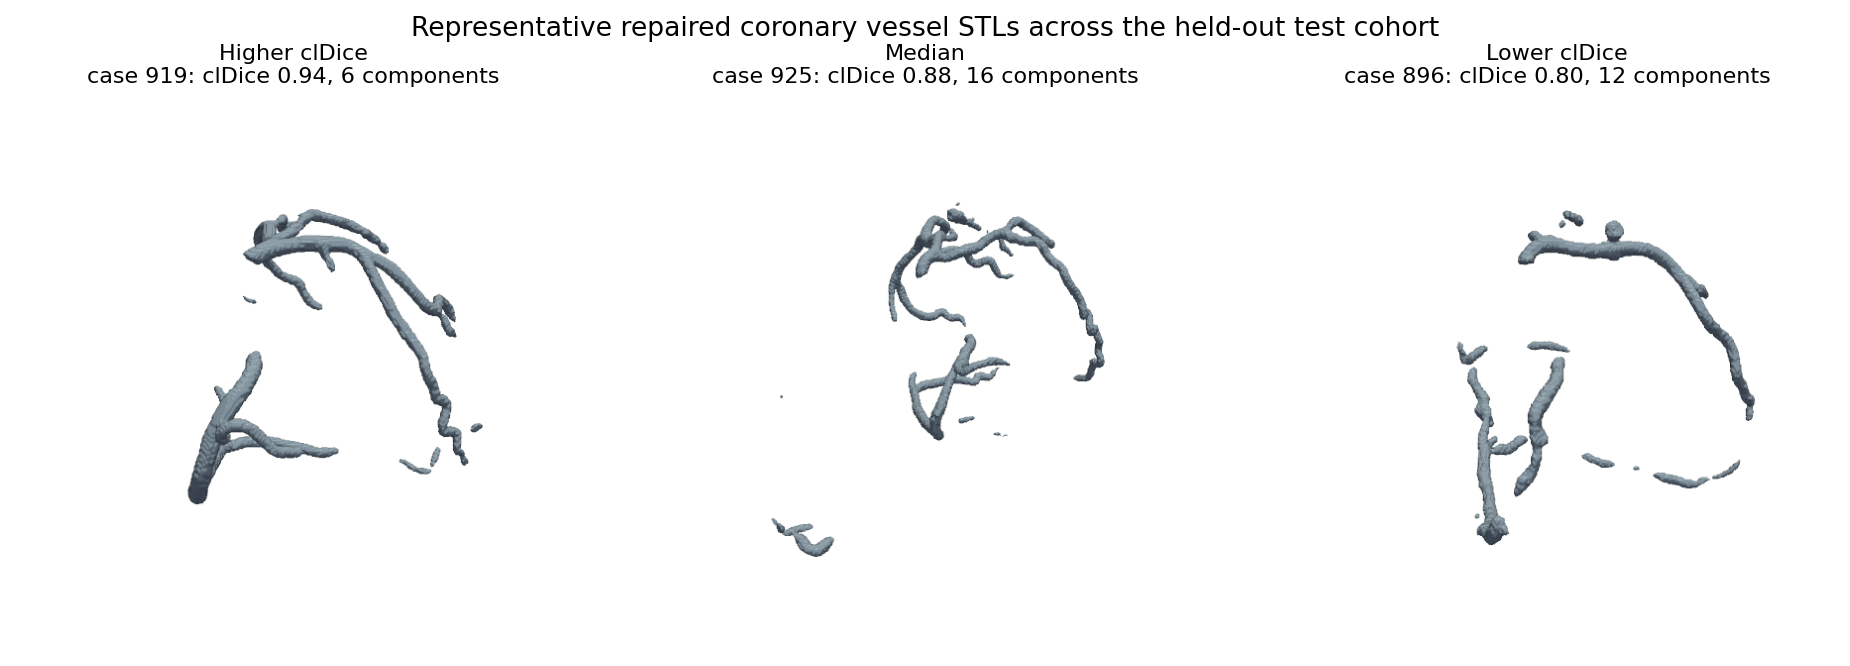
\includegraphics[
        width=0.90\textwidth,
        trim={1.0cm 2.5cm 1.0cm 2.2cm},
        clip
    ]{figure6_vessel_stl_cohort.png}
    \caption{Representative repaired coronary-vessel STLs from three held-out
    test cases spanning the cohort range of topology-aware accuracy: higher,
    median, and lower clDice@0.5. Higher centerline overlap corresponds to
    cleaner, less fragmented vessel trees, consistent with the paired analysis
    in Section~\ref{subsec:paired}.}
    \label{fig:heart-stl}
\end{figure}

\begin{table}[H]
\centering
\caption{Numerical results and run details available from exported project materials.}
\label{tab:results}
\begin{threeparttable}
\footnotesize
\begin{tabularx}{0.92\textwidth}
{L{0.42\textwidth}Y}
\toprule
\textbf{Metric or run detail}
&
\textbf{Reported or derived value}
\\
\midrule
Total samples discovered
&
1000
\\
Training / validation / held-out test split
&
700 / 50 / 250
\\
Final held-out test cases evaluated
&
250
\\
Failed held-out test cases
&
0
\\
Primary test metric
&
Dice@0.5
\\
Test Dice@0.5, mean (95\% CI)
&
0.7878 (0.7820-0.7935)
\\
Test Dice@0.5, median / SD / IQR
&
0.7934 / 0.0461 / 0.0630
\\
Test Dice@0.5, min-max
&
0.6174-0.8696
\\
Test soft Dice, mean (95\% CI)
&
0.7795 (0.7738-0.7852)
\\
Test precision@0.5, mean (95\% CI)
&
0.7636 (0.7554-0.7719)
\\
Test recall@0.5, mean (95\% CI)
&
0.8205 (0.8120-0.8290)
\\
Test HD95@0.5, mean / median
&
\SI{5.01}{mm} / \SI{3.69}{mm}
\\
Test runtime, mean / median (MPS)
&
\SI{196.7}{s} / \SI{199.2}{s} per case
\\
Test clDice@0.5, mean / median (95\% CI)
&
0.8695 / 0.8753 (0.8629-0.8761)
\\
Submitted Attention U-Net parameter count
&
23,625,953 trainable parameters
\\
Training class imbalance
&
78,936,341 positive voxels vs. 47,202,404,075 negative voxels
\\
Corrected negative-to-positive ratio
&
Approximately 598:1
\\
Representative max roughness change
&
\SI{0.237}{mm} to \SI{0.120}{mm}
\\
Representative mean roughness change
&
\SI{0.070}{mm} to \SI{0.044}{mm}
\\
Representative mean roughness improvement
&
37.1\%
\\
Representative Phase B result (case 720)
&
Watertight and single-component after repair; surface area 7854.84\,mm$^2$; volume 7071.36\,mm$^3$; minimum radius \SI{0.355}{mm}; 39.94\% of radii below the \SI{0.6}{mm} proxy; overall computational QC fail
\\
Cohort Phase B mesh QC (250 cases)
&
228/250 (91.2\%) met the combined mesh-integrity criterion; mean 10.2 and median 9 connected components; primary slicability 125/250 (50.0\%); strict all-50-plane slicability 61/250 (24.4\%); two-voxel affine-aware alignment 250/250
\\
Strongest segmentation-mesh association
&
clDice@0.5 vs.\ connected-component count, Spearman $\rho=-0.49$ ($p_\mathrm{FDR}=2.3\times10^{-15}$)
\\
Final test files
&
\texttt{outputs/final\_test\_250/per\_case\_metrics.csv}, \texttt{summary\_metrics.json}, \texttt{seg\_to\_mesh\_correlations.csv}; \texttt{outputs/phase\_b\_mesh\_qc/summary\_mesh\_qc.json}

\\
\bottomrule
\end{tabularx}
\end{threeparttable}
\end{table}



% =========================================================
\section{Discussion}
% =========================================================

\subsection{Principal findings}

The pipeline connects coronary CTA segmentation to fabrication-oriented mesh generation. The full 250-case held-out ImageCAS evaluation supports the segmentation stage. The primary Dice@0.5 result was 0.7878 with a 95\% CI of 0.7820-0.7935, median 0.7934, and zero failed cases, with a topology-aware clDice@0.5 of 0.8695. The mean Dice was just below 0.80. The paired analysis shows centerline-aware accuracy predicts mesh connectivity better than voxel overlap.

\FloatBarrier

The main implication is that image-to-fabrication pipelines should not end just at segmentation metrics. For coronary and vascular structures, distal branch dropout, false bridges, and local discontinuities may have limited effect on Dice but substantially affect geometry. This is especially important for biofabrication, where a disconnected or non-manifold vascular model may fail as a perfusable blueprint even if there is high voxel overlap. The representative Phase B result complements this claim but in an opposite direction, showing that a mesh can be geometrically clean (watertight and single-component) but still unfit for printing because much of coronary geometry is at a sub-millimeter scale. Both observations argue that segmentation accuracy and fabrication readiness must be reported and evaluated as distinct objectives. The present pipeline addresses that gap by generating STL artifacts and QC summaries. The representative PrusaSlicer assessment provides supporting computational evidence of STL-to-toolpath continuity under one fixed reference profile; the clDice--mesh-fragmentation relationship remains the principal scientific finding.

The comparison with ImageCAS-related literature also states the status of the result. The completed held-out test result is comparable to public coronary CTA segmentation work and is now supported by per-case statistics including precision, recall, HD95, the topology-aware clDice, and cohort-level Phase~B mesh QC. Because no external validation was possible, given the shortage of compatible public datasets, the strongest supported claim is that the pipeline is feasible, reproducible in structure, and relevant to future biofabrication workflows.


\subsection{Biofabrication relevance and claim boundary}

Phase~B contributes integration, not new meshing algorithms. Marching cubes and mesh repair are established tools \cite{lorensen1987,lewiner2003}, and their value here is being placed inside a CTA-to-STL workflow that preserves spatial metadata, accepts segmentation probability maps, produces repaired STL output, and records QC artifacts. This matters for a biofabrication audience because the practical barrier is rarely any single algorithm but instead the reliable movement from an image volume to usable geometry.

For biofabrication, patient-specific vascular geometry from imaging is useful in at least three ways: as a template for perfusable-channel design or sacrificial-path planning in engineered tissues \cite{kolesky2014,hinton2015}, as a basis for cardiovascular phantoms or preoperative models, where geometric realism matters, and as a way to standardize the upstream computational workflow that physical printing depends on. The postprocessing choices here are deliberate: affine-aware geometric validation guards against spatial distortion, while mesh repair and QC reporting separate geometric integrity from downstream fabrication claims.

The corrected cohort checks separate geometric integrity (watertightness and detected non-manifold edges), fragmentation, cross-sectional slicability, and affine-aware spatial fidelity. The representative production-slicer demonstration then assesses software-level toolpath generation for one case. These distinct checks form an intermediate computational layer between voxelwise segmentation and physical fabrication without establishing physical printability.

The claim boundary is therefore explicit. These results demonstrate computational preparation of STL geometry from CTA-derived vascular segmentations and representative software-level STL-to-toolpath generation. They do not demonstrate cell-laden printing, perfusion under flow, endothelialization, long-term construct viability, implantation, or clinical readiness; reaching any of those would require cohort-level and bioprinter-specific toolpath validation, physical print trials, and lumen-patency and perfusion testing.


\subsection{Limitations}
Several limitations should be stated explicitly. First, the dataset labels coronary arteries, not the full cardiac vascular hierarchy. The system is therefore a coronary (macrovascular) CTA-to-STL pipeline, not a microvascular reconstruction method. Second, the study is entirely computational and reports no physical bioprinting, mechanical testing, perfusion assay, or biological validation. Third, evaluation is confined to a single dataset (ImageCAS), and external validation on independent coronary CTA data is still needed. Fourth, although clDice and the paired analysis show that topology tracks mesh connectivity, overlap-based metrics alone, voxel or centerline, cannot establish distal-branch continuity, lumen preservation, or print readiness. Fifth, cohort-level and bioprinter-specific toolpath validation was not established; the production-slicer assessment was limited to one representative case, and no physical printer or physical fabrication was used. Bioink compatibility, lumen patency, perfusion, mechanical behavior, quantitative surface fidelity, and biological function were not evaluated. Sixth, component counts above the two-vessel anatomical baseline were common (median 9), consistent with the clDice-fragmentation relationship in Section~\ref{subsec:paired}; connected-component filtering, already supported in the implementation but not applied here, is a straightforward next step toward single-tree exports.

\subsection{Future validation priorities}

Because coronary arteries form connected tubular networks, preservation of vessel continuity is often more important for fabrication than voxel-wise overlap alone. For this reason, we report topology-aware metrics such as clDice and connected-component behavior in addition to Dice. More detailed centerline-based measures, including centerline distance, branch-detection accuracy, and distal-vessel recall \cite{shit2021}, would provide a finer assessment of continuity on a branch-by-branch basis.

The clearest gap on the modeling side is the absence of a head-to-head baseline. A plain 3D U-Net or an nnU-Net reference, trained and evaluated under the same split, preprocessing, and inference settings, would benchmark the result directly instead of only placing it against published numbers.

The representative PrusaSlicer demonstration establishes software-level toolpath generation for case 720 under one fixed reference profile. Remaining work includes cohort-level production-slicer validation, bioprinter-specific toolpath generation, bioink- and material-aware parameterization, physical printing, quantitative geometric print-fidelity testing, and mechanical, perfusion, and biological evaluation where appropriate. External validation should accompany these downstream studies.

% =========================================================
\section{Conclusion}
% =========================================================

This study presents an integrated computational pipeline that converts coronary CT angiography into segmentation-derived, bioprinting-oriented vascular STL models. On the complete 250-case held-out ImageCAS test set, the three-dimensional Attention U-Net achieved a mean Dice score of 0.7878 and a mean topology-aware clDice score of 0.8695, with successful inference across all cases. The Phase B workflow completed mesh extraction and repair for the full cohort, with 91.2\% meeting the combined watertight and zero-detected-non-manifold-edge criterion and all 250 meshes meeting the two-voxel affine-aware alignment criterion.

The study also shows the value of evaluating vascular models as a joint segmentation-to-geometry problem. Topology-aware clDice showed a stronger association with reduced mesh fragmentation than Dice did. This finding supports the use of centerline-sensitive evaluation when preparing complex vascular geometries for biofabrication workflows.

By combining coronary segmentation, topology-aware evaluation, mesh reconstruction, repair, and automated quality-control reporting in a single reproducible framework, the pipeline covers the image-to-mesh steps between medical imaging and biofabrication that usually require manual work. Representative production-slicer toolpath generation was also demonstrated for case 720 under a fixed reference profile, without physical printing. The workflow can support fabrication planning, sacrificial-channel design, and later experimental validation of image-derived vascular geometries.

\section*{Data and code availability}

The completed held-out test outputs are retained in \texttt{outputs/final\_test\_250/} with per-case results, summary metrics, evaluation logs, configuration files, and paired-analysis outputs. Corrected cohort mesh-quality, slicability, centroid, and alignment results are retained in \texttt{outputs/phase\_b\_mesh\_qc/}; \texttt{run\_missing\_checks.py} reproduces the lightweight checks when the excluded case-level masks and meshes are available. The representative production-slicer workflow and compact case-720 evidence are retained in \texttt{production\_slicer\_validation.py} and \texttt{outputs/production\_slicer\_validation/}. The evaluation can be reproduced from the checkpoint \texttt{checkpoints/best\_dice05.pt} using the orchestration script \texttt{run\_full\_revision.sh}. Together, these artifacts support verification of the reported held-out test, clDice, mesh-QC, paired-analysis, and representative toolpath results. The per-epoch training log for the evaluated checkpoint was not retained (Section~\ref{subsec:training-convergence}).

The implementation was developed in Python using PyTorch, MONAI, NumPy, SciPy, NiBabel, pandas, and related medical image-processing libraries. To support double-anonymous review, the manuscript, code, and derived results were anonymized. An anonymized code and results archive will be provided during review or upon reasonable request, subject to dataset-use restrictions. User-specific paths, usernames, email addresses, and institutional identifiers were removed from the codebase, logs, figures, and manuscript materials.

\section*{Declarations}

\textbf{Ethics.} This study used de-identified public imaging data and did not involve new human-subject recruitment, intervention, clinical deployment, animal experimentation, or collection of private patient data.

\textbf{Competing interests.} The authors declare no competing interests.

\textbf{Acknowledgements.} Author names, institutional identifiers, and funding details have been removed for double-anonymous review and can be restored after peer review if requested by the journal.

\appendix

\section{Reproducibility details}
\label{app:repro}

\subsection*{A.1\quad Training-time augmentation parameters}

Table~\ref{tab:aug} lists the training-time augmentations used by the evaluated model, together with their order, sampling probabilities, and parameter settings. Intensity augmentations operate on images scaled to $[0,1]$. Spatial augmentations are applied jointly to images and labels, with nearest-neighbor interpolation used for labels. Preprocessing steps shared by training, validation, and inference are described in Section~\ref{subsec:dataset} and are not repeated here.

\begin{table}[!htbp]
\centering
\caption{Training-time data-augmentation transforms (MONAI dictionary transforms), in execution order, as used for the evaluated model. Probabilities and parameters are read directly from the training configuration. Elastic deformation is implemented but was disabled for the reported run.}
\label{tab:aug}
\small
\begin{tabularx}{\textwidth}{@{}l l Y@{}}
\toprule
Transform (MONAI) & Probability & Parameters \\
\midrule
\texttt{SpatialPadd} & 1.0 & target $96\times192\times192$ \\
\texttt{RandCropByPosNegLabeld} & --- & pos:neg $=3{:}1$, num\_samples $=2$, allow\_smaller, image\_threshold $=0$ \\
\texttt{RandFlipd} & 0.5 & spatial\_axis $=[0,1,2]$ \\
\texttt{RandRotate90d} & 0.5 & max\_k $=3$ \\
\texttt{RandRotated} & 0.1 & range\_x/y/z $=\pm0.2$ rad ($\approx\pm11.5^\circ$); mode (bilinear, nearest) \\
\texttt{Rand3DElasticd} & disabled & implemented as $p=0.2$, sigma\_range $(4,6)$, magnitude\_range $(50,150)$; not applied \\
\texttt{RandAdjustContrastd} & 0.4 & gamma $\in[0.8,1.2]$ \\
\texttt{RandScaleIntensityd} & 0.5 & factors $=(0.85,1.15)$ \\
\texttt{RandShiftIntensityd} & 0.3 & offsets $=0.1$ \\
\texttt{RandGaussianNoised} & 0.2 & mean $=0.0$, std $=0.01$ \\
\texttt{RandGaussianSmoothd} & 0.3 & sigma\_x/y/z $=(0.5,1.5)$ \\
\texttt{ResizeWithPadOrCropd} & 1.0 & target $96\times192\times192$ \\
\bottomrule
\end{tabularx}
\end{table}
\subsection*{A.2\quad Per-case results table}

Per-case test results are provided in \texttt{outputs/final\_test\_250/per\_case\_metrics.csv}, with one row per test case. Each row contains the case identifier, image and label paths, evaluation status, soft Dice score, ground-truth foreground voxel count, and runtime.
Metrics reported at the evaluation threshold of $0.5$ include Dice, precision, recall, false-positive voxel count, false-negative voxel count, predicted voxel count, 95th-percentile Hausdorff distance (HD95; mm), and clDice.
When Phase~B QC is enabled, additional mesh-quality metrics are included, such as connected-component count, watertightness, non-manifold edge count, repair status, surface roughness, minimum-radius proxy, and wall-thickness compliance.

\subsection*{A.3\quad Training and mesh-generation hyperparameters}

Table~\ref{tab:hparams} consolidates the numerical settings for the evaluated checkpoint (Phase~A training and inference) and for the Phase~B mesh-generation run that produced the cohort results in Table~\ref{tab:phaseb-qc}. Values are taken directly from the training and Phase~B source and the exported run configuration; settings not listed used framework defaults.

\begin{table}[H]
\centering
\caption{Consolidated Phase~A and Phase~B hyperparameters for the evaluated checkpoint and reported mesh cohort.}
\label{tab:hparams}
\begin{threeparttable}
\scriptsize
\renewcommand{\arraystretch}{0.88}
\begin{tabularx}{0.92\textwidth}{L{0.46\textwidth}Y}
\toprule
\textbf{Parameter} & \textbf{Value} \\
\midrule
\multicolumn{2}{@{}l}{\textit{Optimization}}\\
Optimizer & AdamW \\
Learning rate & $2\times10^{-5}$ \\
Weight decay & $1\times10^{-5}$ \\
Max epochs / early-stopping patience & 100 / 15 \\
Best (checkpointed) epoch & 79 \\
Gradient clipping (L2 norm) & 1.0 \\
Batch size / gradient accumulation & 1 / 2 (effective 2) \\
Random seed & 42 \\
LR scheduler & ReduceLROnPlateau (mode $=$ max on val Dice@0.5) \\
\quad factor & 0.5 \\
\quad patience & 6 \\
\quad minimum LR & 0 (PyTorch default; not set) \\
\addlinespace
\multicolumn{2}{@{}l}{\textit{Loss} (Eq.~\ref{eq:loss})}\\
Term weights (Tversky / Dice / downsampled Tversky) & 0.6 / 0.4 / 0.3 \\
Tversky $\alpha$ (FN) / $\beta$ (FP) & 0.7 / 0.3 \\
Auxiliary-supervision downsampling & $2\times$ (\texttt{avg\_pool3d}, kernel 2, stride 2) \\
Tversky / Dice smoothing constant & $1\times10^{-5}$ \\
\addlinespace
\multicolumn{2}{@{}l}{\textit{Sampling and inference}}\\
Patch size & $96\times192\times192$ \\
Positive:negative patch ratio & 3:1 (2 samples/case) \\
Sliding-window overlap & 0.625 \\
Binarization threshold & 0.5 \\
\addlinespace
\multicolumn{2}{@{}l}{\textit{Phase~B mesh generation} (corrected reported cohort)}\\
Isosurface & marching cubes, Lewiner variant, isovalue 0.5 \\
Scalar-field pre-smoothing / supersampling / padding & none \\
Mesh repair & \texttt{fix\_normals}, \texttt{fill\_holes} \\
World-coordinate mapping & Complete NIfTI affine to RAS (orientation/reflection, translation, and spacing) \\
Taubin smoothing & Not applied in the corrected 250-case validation; illustrative case-720 analysis only \\
Connected-component filtering & none (all retained; count reported) \\
Slicability & 50 planes normal to the longest bounding-box axis; primary and strict definitions reported separately \\
Spatial alignment & Mesh/mask world-coordinate bounding boxes within two voxels \\
Watertightness & \texttt{trimesh.is\_watertight} \\
\addlinespace
\multicolumn{2}{@{}l}{\textit{Statistics}}\\
95\% confidence interval & normal approximation, $\bar{x}\pm 1.96\,s/\sqrt{N}$ ($s$: sample SD, ddof $=1$; $N$: per-metric case count); verified against a 10{,}000-resample percentile bootstrap, which agreed to three decimal places on all reported metrics \\
\bottomrule
\end{tabularx}
\begin{tablenotes}\footnotesize
\item Unlisted scheduler arguments (threshold, cooldown, $\varepsilon$) and unlisted marching-cubes arguments used framework defaults.
\end{tablenotes}
\end{threeparttable}
\end{table}

\section{Model-provenance record}
\label{app:provenance}

The held-out test metrics were obtained by re-evaluating the 250-case test partition using the best saved checkpoint, which achieved a validation Dice@0.5 of $0.7889$ and a soft Dice of $0.7811$. Complete optimizer, scheduler, configuration, and git-commit metadata were available for this run. Inference used a sliding-window approach (ROI $96\times192\times192$, overlap $0.625$, threshold 0.5). The evaluation completed with 0 failed cases and achieved a mean Dice@0.5 of $0.7878$. The checkpoint was loaded using strict state-dict matching, with no missing or unexpected keys, confirming compatibility with the model architecture (MONAI Attention U-Net, channels $(32,64,128,256,512)$, dropout 0.1). The evaluation was performed on Apple M4 Pro (MPS) hardware. Since inference and metric computation are deterministic, the reported overlap and topology statistics are numerically close but not bitwise identical relative to CUDA execution.

\section{Code Availability}
The code with both Phase A and Phase B can be found at \url{https://github.com/myalageri22/Automated_Cardiovascular_Segmentation_Bioprinting}.


\newpage
\bibliographystyle{iopart-num}
\bibliography{references}

\end{document}
